\section{Eliminating Time Shortcuts: Paired Causal Visual Audit}
\label{sec:diagnosis}

Before designing multimodal graph architectures or training fusion networks, we first construct an uncontaminated diagnostic environment on \texttt{NED}~\cite{lin2024ned} to measure precisely when images rescue ambiguous posts versus when they cause false merges.

\subsection{Time-Shortcut Removal and Event-Split Isolation}
\label{sec:setup_splits}

We adopt the pre-registered seed-$20261106$ stratified split of the 40 \texttt{NED} events into three strictly disjoint sets covering matched topic diversity (sports, weather, earthquake, violence, politics, fire):
\begin{itemize}
    \item \textbf{Development (Gate~B only):} 8 events (\texttt{E15, E23, E22, E33, E40, E11, E24, E38}; $2{,}665$ posts; $2{,}131$ valid decoded images), forming four concurrent same-theme competing pairs (\texttt{E15}$\leftrightarrow$\texttt{E23}, \texttt{E22}$\leftrightarrow$\texttt{E33}, \texttt{E38}$\leftrightarrow$\texttt{E40}, \texttt{E11}$\leftrightarrow$\texttt{E24});
    \item \textbf{Validation:} 8 events (\texttt{E25, E26, E19, E20, E9, E36, E6, E31}; $2{,}746$ posts; $1{,}950$ valid decoded images), used solely for calibrating clustering/routing thresholds and verifying robustness prior to locking the protocol;
    \item \textbf{Held-Out Test:} 24 unseen events ($11{,}955$ posts; $9{,}311$ valid decoded images), remaining completely untouched until after freezing \texttt{protocol\_trackB\_v1.json}.
\end{itemize}
To eliminate the chronological $72$-hour separation shortcut ($B^3\text{-}F_1 = 0.9900$), every post $i$ inside event $E(i)$ receives an event-relative timestamp $\tau^{\text{rel}}_i = \tau_i - \min_{j \in E(i)} \tau_j$, aligning all events concurrently from $t=0$ with zero temporal edge decay ($\lambda_\tau = 0$). Neither \texttt{event\_name} strings nor raw calendar dates/years are ever exposed to text encoders or VLM prompts. Moreover, to guarantee visual rescues do not arise from memorizing duplicated photos across posts, we compute a 64-bit difference hash (\texttt{dHash64}) for each image and filter Tier~1A and Tier~2 evaluation strictly to \emph{novel} non-duplicate query images whose Hamming distance to all cluster anchor images satisfies $\mathrm{dHash}(\cdot,\cdot) > 6$ ($1{,}527$ of $1{,}589$ query posts on \texttt{development}; only $1.0\%$ of development images share exact \texttt{dHash64}).

\subsection{Three-Condition Counterfactual Protocol}
\label{sec:paired_protocol}

Each development event's earliest $25\%$ posts form unlabeled candidate cluster anchors summarized strictly by top-$5$ hashtags/tokens and $3$ central medoids. For every novel query post $m_i = (x_i, v_i)$ facing a 4-way candidate set $\mathcal{C}_{\text{cand}}(i)$ containing its true event, its same-theme competitor, and top-$2$ nearest concurrent alternatives, we evaluate each scorer/VLM under three paired visual interventions while fixing $x_i$ and $\mathcal{C}_{\text{cand}}(i)$:
\begin{enumerate}
    \item \textbf{\texttt{Text-Only}:} visual modality masked ($x_i$ only);
    \item \textbf{\texttt{Orig-Img}:} original post pair $(x_i, v_i)$;
    \item \textbf{\texttt{Mismatched-Img}:} text $x_i$ paired with a non-duplicate image $v'_j$ ($\mathrm{dHash} > 6$) drawn from the competing same-theme event.
\end{enumerate}
Let $c^{\text{txt}}_i, c^{\text{orig}}_i, c^{\text{mis}}_i \in \{0,1\}$ denote correctness under the three conditions against ground truth $y_i$. We directly measure:
\begin{equation}
\label{eq:rescue_mislead}
\begin{aligned}
N_{\text{rescue}} &= \sum_i \mathbb{I}[c^{\text{txt}}_i = 0 \wedge c^{\text{orig}}_i = 1], \qquad
N_{\text{mislead}} = \sum_i \mathbb{I}[c^{\text{txt}}_i = 1 \wedge c^{\text{orig}}_i = 0], \\
N_{\text{misflip}} &= \sum_i \mathbb{I}[c^{\text{txt}}_i = 1 \wedge c^{\text{mis}}_i = 0].
\end{aligned}
\end{equation}
In Tier~1A, we audit linear cosine fusion $s_{\text{txt}} + \lambda_V b_i s_{\text{vis}}$ ($\lambda_V = 0.75$) over frozen \texttt{all-MiniLM-L6-v2} text prototypes~\cite{reimers2019sentence} and \texttt{CLIP ViT-B/32} image prototypes~\cite{radford2021clip} across all $n=1{,}527$ novel queries at zero API cost, comparing \texttt{Visual-IDF} ($b_i = \ln 2 / \ln(2 + \#\{j : \cos(v_i, v_j) \ge 0.88\})$), \texttt{CNTD-Raw} (penalizing caption cosine dispersion across top-8 visual neighbors with $\cos \ge 0.65$), \texttt{CNTD-Cond} (penalizing only near-orthogonal conflicts $\cos < 0.12$ scaled by \texttt{Visual-IDF}), and prototype \texttt{Comp-Margin}. In Tier~1B, we run concurrent unsupervised multi-view 2D-SE clustering over all $2{,}665$ dev posts. In Tier~2, we run $120$ stratified novel-image posts $\times 3$ conditions $= 360$ live calls on \texttt{Qwen/Qwen3-VL-8B-Instruct} ($360/360$ \texttt{HTTP 200 OK}, $312{,}713$ prompt + $20{,}065$ completion $= 332{,}778$ real tokens, $1{,}446.1\text{ s}$) eliciting explicit structured flags \texttt{visual\_discriminative} and \texttt{visual\_conflict\_with\_text}.

\begin{table*}[t]
\centering
\caption{Gate~B Three-Condition Counterfactual Visual Audit on Concurrent \texttt{NED Development} (Non-Duplicate Novel Images: Tier~1A CLIP $n=1{,}527$, $\lambda_V=0.75$; Tier~2 \texttt{Qwen/Qwen3-VL-8B-Instruct} $n=120 \times 3 = 360$ OK calls). Bold highlights best column trade-off.}
\label{tab:gateb_summary}
\resizebox{\textwidth}{!}{%
\begin{tabular}{llcccccccc}
\toprule
\textbf{Audit Tier} & \textbf{Visual Evidence Policy} & \textbf{Text Acc.} & \textbf{Orig Acc.} & \textbf{Orig Macro-$F_1$} & \textbf{Mismatch Acc.} & \textbf{$N_{\text{rescue}}$} & \textbf{$N_{\text{mislead}}$} & \textbf{Net ($\Delta$)} & \textbf{$N_{\text{misflip}}$} \\
\midrule
\multirow{7}{*}{Tier 1A: CLIP ($n=1{,}527$)}
& Text-Only Baseline & 0.8271 & 0.8271 & 0.8196 & 0.8271 & +0 & 0 & +0 & 0 \\
& Naive Visual & 0.8271 & \textbf{0.8723} & \textbf{0.8752} & 0.7439 & \textbf{+96} & 27 & \textbf{+69} & 158 \\
& Visual-IDF & 0.8271 & 0.8684 & 0.8684 & 0.7570 & +90 & 27 & +63 & 135 \\
& CNTD-Raw (Dispersion Penalty) & 0.8271 & 0.8553 & 0.8599 & \textbf{0.7917} & +59 & 16 & +43 & 76 \\
& CNTD-Cond (Conflict + Vis-IDF) & 0.8271 & 0.8657 & 0.8634 & 0.7603 & +85 & 26 & +59 & 130 \\
& Comp-Margin & 0.8271 & 0.8540 & 0.8542 & 0.7570 & +50 & \textbf{9} & +41 & 135 \\
& Comp-Margin (Text-Conf Guard) & 0.8271 & 0.8540 & 0.8542 & 0.7839 & +50 & \textbf{9} & +41 & 78 \\
\midrule
\multirow{6}{*}{Tier 2: \texttt{Qwen3-VL-8B} ($n=120$)}
& \texttt{vlm\_text\_only} & 0.7500 & 0.7500 & 0.8378 & \textbf{0.7500} & 0 & 0 & +0 & 0 \\
& \texttt{vlm\_naive\_orig} & 0.7500 & 0.8333 & 0.9075 & 0.1167 & \textbf{17} & 7 & +10 & 77 \\
& \texttt{vlm\_visual\_idf\_gate} & 0.7500 & 0.8250 & 0.9038 & 0.1167 & 16 & 7 & +9 & 77 \\
& \texttt{vlm\_cntd\_raw\_gate} & 0.7500 & 0.7750 & 0.8646 & 0.1167 & 7 & 4 & +3 & 77 \\
& \textbf{\texttt{vlm\_self\_gate}} ($\text{disc} \wedge \neg\text{conflict}$) & 0.7500 & \textbf{0.8500} & \textbf{0.9097} & 0.7083 & 12 & \textbf{0} & \textbf{+12} & \textbf{5} \\
& \textbf{\texttt{vlm\_comp\_evid\_gate}} (+Conf Guard) & 0.7500 & 0.8250 & 0.9022 & \textbf{0.7500} & 9 & \textbf{0} & +9 & \textbf{0} \\
\bottomrule
\end{tabular}}
\end{table*}

\begin{figure*}[t]
  \centering
  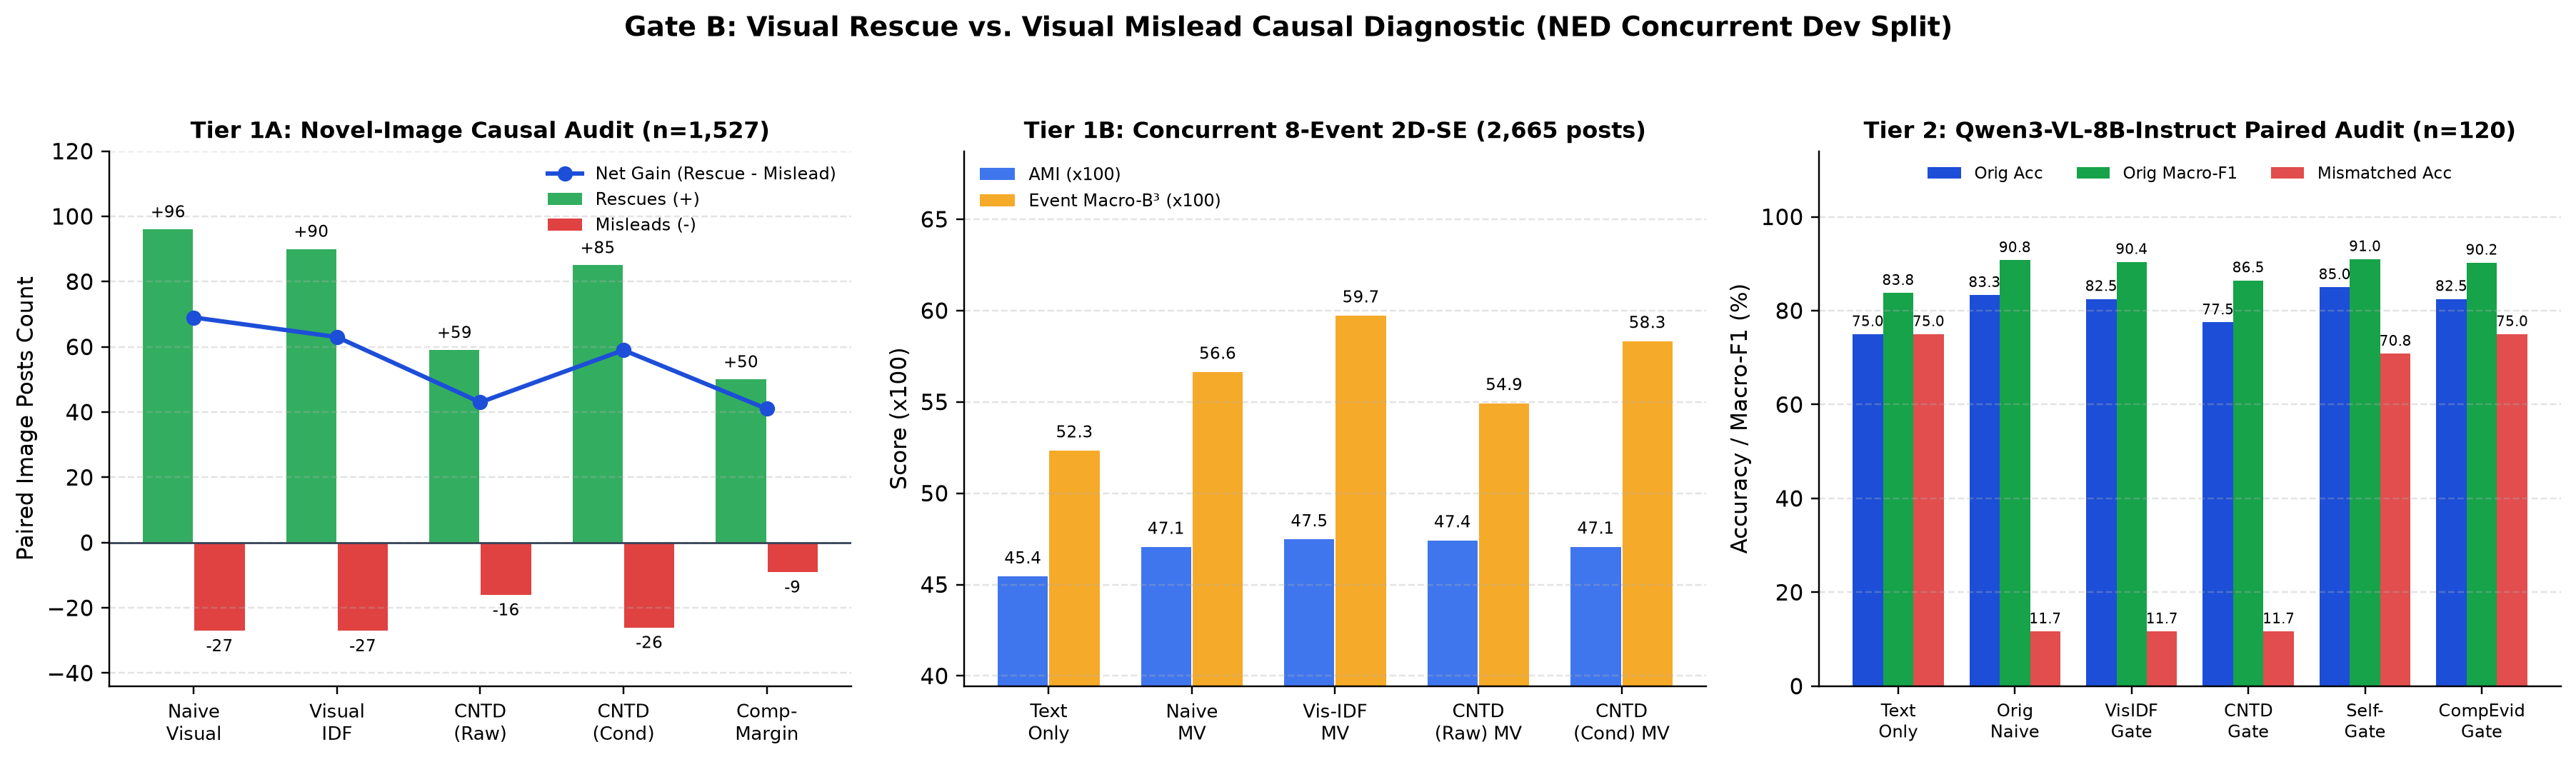
\includegraphics[width=0.98\textwidth]{figures/gateB_ned_dev_qwen3_vl_8b.png}
  \caption{Gate~B causal diagnostic on concurrent \texttt{NED Development}: (left) Tier~1A novel-image rescues vs.\ misleads; (middle) Tier~1B concurrent 2D-SE clustering across $2{,}665$ posts; (right) Tier~2 \texttt{Qwen/Qwen3-VL-8B-Instruct} paired audit confirming \texttt{Self-Gate} ($85.0\%$ Orig, $0$ misleads, $77 \to 5$ mismatch flips) and \texttt{CompEvid-Gate} ($75.0\%$ mismatch floor, $0$ flips).}
  \label{fig:gateb}
\end{figure*}

\subsection{Key Causal Findings and Design Lessons}
\label{sec:gateb_findings}

Table~\ref{tab:gateb_summary} and Figure~\ref{fig:gateb} establish four empirical facts that govern our architecture:
\begin{enumerate}
    \item \textbf{Dual Phenomena Are Real on Non-Duplicate Images:} Under naive fusion, real concurrent images rescue $+96$ (Tier~1A) and $+17$ (Tier~2) text-ambiguous posts, yet simultaneously introduce $27$/$7$ natural original misleads and catastrophic competing-image hijacking ($158$ flips in Tier~1A; $77$ flips plunging VLM accuracy from $75.00\%$ to $11.67\%$ in Tier~2).
    \item \textbf{Refutation of \texttt{CNTD-Raw} Across All Three Levels:} Penalizing cross-neighbor caption dispersion cuts legitimate rescues in half ($+96 \to +59$ in Tier~1A; $17 \to 7$ in Tier~2), slashes concurrent 2D-SE Event Macro-$B^3$ by $-4.80\text{ pp}$ ($0.5973 \to 0.5493$, increasing false merges with $\text{net\_fm\_red} = -996$ vs.\ $-38$), and fails to block VLM competing-image hijacks ($77$ flips, $11.67\%$).
    \item \textbf{Graph \texttt{Visual-IDF} Helps Unsupervised Clustering Yet Misses Unique Distractors:} In Tier~1B concurrent 2D-SE ($2{,}665$ posts), \texttt{visual\_idf\_mv\_2dse} elevates Event Macro-$B^3$ by $+7.39\text{ pp}$ over text-only 2D-SE ($0.5234 \to 0.5973$; AMI $0.4544 \to 0.4747$; $K=118 \to 98$, eliminating $32{,}792$ false-split pairs). However, sample-level distractors in Tier~2 are visually unique (\texttt{Visual-IDF} $= 1.000$), leaving \texttt{vlm\_visual\_idf\_gate} exposed ($7$ original misleads, $77$ mismatch flips). Moreover, static frozen CLIP \texttt{Comp-Margin} divided by $0.10$ over-damped typical $0.02$--$0.05$ CLIP prototype margins, dropping Tier~1A rescues from $+96$ to $+50$ and Tier~1B Macro-$B^3$ from $0.5973$ to $0.5442$.
    \item \textbf{Cross-Modal Conflict Gating Resolves Both Regimes:} \texttt{Qwen/Qwen3-VL-8B-Instruct} flags \texttt{visual\_conflict\_with\_text} $= \text{True}$ on $16/120$ original images and $99/120$ mismatched competing images. Gating visual adoption on \texttt{visual\_discriminative} $\wedge \neg\texttt{visual\_conflict\_with\_text}$ (\texttt{vlm\_self\_gate}) raises original accuracy to $85.00\%$ ($+10.00\text{ pp}$ over text-only; $0$ misleads) and reduces mismatch flips $77 \to 5$ ($70.83\%$); adding competitor/confidence guards (\texttt{vlm\_comp\_evid\_gate}) achieves \textbf{zero misleads and zero mismatch flips} ($82.50\%$ original / $75.00\%$ mismatched).
\end{enumerate}

\paragraph{Concrete Micro-Cases.}
Inspection confirms exact mechanisms: (i) \emph{True Rescues (\texttt{Visual-IDF} $=1.0$):} \texttt{ned\_05292} carries only generic text \emph{``Live| Evacuation of detainees from the stadium after the explosion!''} (\texttt{Text-Only} $= \text{NEW}$), yet its photo of night police and barriers restores it to \texttt{E11}; \texttt{ned\_09331} (Volunteers clearing downed poles/trees) and \texttt{ned\_09280} (Guard cargo plane pallets) rescue text-ambiguous \texttt{E22} posts while triggering \texttt{visual\_conflict} $= \text{True}$ when swapped with flooded Japanese train imagery. (ii) \emph{Natural Misleads \& Hijacks:} \texttt{ned\_05166} (\texttt{\#Prayers4Paris} + Scottish flag), \texttt{ned\_09302} (\texttt{\#PrayForPuertoRico} + white dog), and \texttt{ned\_09610} (\texttt{ASTROS WIN} + man holding book) all flip to \texttt{NEW} under naive VLM and are blocked by our gate; strikingly, \texttt{ned\_09980} (\emph{``Fall Classic''}, \texttt{E23}) swaps from Minute Maid Park to Wrigley Field under \texttt{Mismatched-Img} and is hijacked directly to the competing World Series event \texttt{E15} unless gated, while \texttt{ned\_05343} (\texttt{\#prayforparis}) flips to \texttt{E24} under an Iranian flag protest photo.
